% id: 0344
% book: 쎈 중3-2 수학 · 03 원과 직선
% section: 유형 11 원의 접선의 성질의 활용
% figure: tikz:fig-0344
% answer: ②
% answer_source: 답지
% variant_level: 0 (원본 전사)
% 이 파일은 build.mjs 가 items.json 에서 만든다. 고칠 때는 items.json 을 고친다.
\smash{\raisebox{1.5mm}{\dmkichul{쎈 중3-2 수학 0344번 · 65쪽}}}
\noindent\begin{minipage}[t]{0.58\linewidth}\vspace{0pt}\raggedright 오른쪽 그림에서 $\seg{CP}$, $\seg{CQ}$, $\seg{AB}$는 각각 점~$\pt{P}$, $\pt{Q}$, $\pt{R}$에서 원~$\pt{O}$에 접한다. $\seg{OP}=6\,\mathrm{cm}$, $\seg{OC}=12\,\mathrm{cm}$일 때, $\triangle\pt{ABC}$의 둘레의 길이는?\end{minipage}\hfill\begin{minipage}[t]{0.4\linewidth}\vspace{0pt}\centering \resizebox{\ifdim\width>\linewidth\linewidth\else\width\fi}{!}{% 0344(본책 65쪽) — CP, CQ, AB 가 P, Q, R 에서 원 O 에 접함, OP=6 cm, OC=12 cm. 답(△ABC 둘레)은 적지 않는다. 스캔 삽화를 TikZ 로 다시 그림.
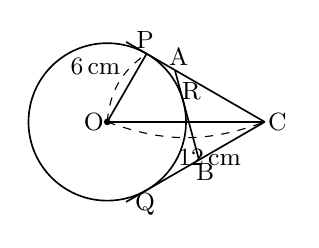
\begin{tikzpicture}[line width=0.6pt]
  \draw (0.000,0.000) circle (1.000);
  \draw (2.000,0.000) -- (0.240,1.016);
  \draw (2.000,0.000) -- (0.240,-1.016);
  \draw (0.859,0.659) -- (1.165,-0.482);
  \draw (0.000,0.000) -- (0.500,0.866);
  \draw (0.000,0.000) -- (2.000,0.000);
  \fill (0.000,0.000) circle (1.2pt);
  \draw[dashed, line width=0.4pt] (0.000,0.000) to[bend left=25] (0.500,0.866);
  \node[font=\small, inner sep=1.5pt] at (-0.150,0.700) {$6\,\mathrm{cm}$};
  \draw[dashed, line width=0.4pt] (0.000,0.000) to[bend right=20] (2.000,0.000);
  \node[font=\small, inner sep=1.5pt] at (1.300,-0.450) {$12\,\mathrm{cm}$};
  \node[font=\small, inner sep=1.5pt] at (-0.170,0.000) {O};
  \node[font=\small, inner sep=1.5pt] at (0.480,1.036) {P};
  \node[font=\small, inner sep=1.5pt] at (0.480,-1.046) {Q};
  \node[font=\small, inner sep=1.5pt] at (0.909,0.829) {A};
  \node[font=\small, inner sep=1.5pt] at (1.245,-0.642) {B};
  \node[font=\small, inner sep=1.5pt] at (1.066,0.399) {R};
  \node[font=\small, inner sep=1.5pt] at (2.160,0.000) {C};
\end{tikzpicture}
}\end{minipage}\par
\begin{choices32}{\rule[-3ex]{0pt}{8ex}$12\sqrt{2}\,\mathrm{cm}$}{\rule[-3ex]{0pt}{8ex}$12\sqrt{3}\,\mathrm{cm}$}{\rule[-3ex]{0pt}{8ex}$24\,\mathrm{cm}$}{\rule[-3ex]{0pt}{8ex}$12\sqrt{5}\,\mathrm{cm}$}{\rule[-3ex]{0pt}{8ex}$12\sqrt{6}\,\mathrm{cm}$}\end{choices32}
